%------------------------------------------------- Chapter --------------------------------------------------------
\parskip=1cm

%\chapter{xxxxxxxxxxxxxxxxxxxx} \label{cap:contratosz} \label{cap:5z}
%\pagenumbering{arabic}
\chapter{Contratos sensibles al contexto}\label{cap:contratos} \label{cap:5}
%\chapter{Framewrok to Implemet Context Aware Contract in E-learning

%\pagenumbering{arabic}

\lstset{style=mystyle}

\section {Introducción}\label{sec:Introducción}


En este capítulo, se comienza a trabajar en el nivel técnico de diseño del artefacto de software principal de la arquitectura arqDHD, que se describe en detalle en el capítulo \ref{cap:arqdhd}. El objetivo principal de este capítulo es desarrollar el contratoDHD, que será una parte fundamental de la arquitectura arqDHD.

Para lograr este objetivo, se comienza con la definición de conceptos importantes que permitirán caracterizar cuestiones de diseño a tener en cuenta en el desarrollo del contratoDHD. Estos conceptos incluyen aspectos técnicos y funcionales que deben ser considerados para garantizar que el contratoDHD cumpla con los requisitos de calidad, rendimiento y funcionalidad.

Una vez establecidos estos conceptos, se procede a identificar los elementos y relaciones necesarios para el diseño del contratoDHD. Para ello, se siguen los lineamientos de diseño para el cambio dinámico utilizados en la arqDHD, que permiten adaptar la arquitectura a los cambios en los requisitos y necesidades del sistema.

Siguiendo el camino hacia la implementación del contratoDHD, se construirán soluciones de diseño de componentes más refinadas para lograr una mejor comprensión en las etapas posteriores de generación de código de implementación. Estas soluciones se basarán en las decisiones de diseño tomadas previamente y en la retroalimentación proporcionada por la implementación del contratoDHD. De esta forma, se asegurará que el diseño final del contratoDHD esté bien adaptado a los requisitos específicos del sistema y cumpla con los estándares de calidad y rendimiento esperados.


\section {Hacia la definición de ContratoDHD}\label{sec:Hacia_la_definición_de_ContratosDHD}

En software, un contrato es un componente que contiene información necesaria sobre las posibilidades de  instanciaciones y relaciones de otras componentes de un sistema. Esta información está construida con condicionales y acciones que pueden ser evaluados en tiempo de ejecución en un sistema. Esto significa que la instancia de un sistema, en un determinado contexto (tiempo, locación, tipo de acción, ejecución, estado del entorno, etc.), dependerá de la información pre-establecida en los contratos. 


El contrato puede ser configurado por medio de diferentes mecanismos. Desde el lenguaje cotidiano hasta un lenguaje de especificación formal, por ejemplo, basado en XML\footnote {XML, sigla en inglés de textit{eXtensible Markup Language} (lenguaje de marcas extensible), es un metalenguaje extensible de etiquetas desarrollado por el World Wide Web Consortium (W3C).} 

%Es una simplificación y adaptación del SGML que permite definir la gramática de lenguajes específicos (de la misma manera que HTML es a su vez un lenguaje definido por SGML). Por lo tanto XML no es realmente un lenguaje en particular, sino una manera de definir lenguajes para diferentes necesidades. Algunos de estos lenguajes que usan XML para su definición son XHTML, SVG, MathML.} para los casos que sean necesarias especificaciones que puedan ser procesadas por máquinas.
%\subsection{Características que debe cumplir el ContratoDHD}

El tipo de tecnología y forma de implementación de los contratos es transparente para los componentes que realizan peticiones, o necesitan información, de otra componente a la que se encuentra relacionada. A esta componente se la podría denominar cliente. Esta relación (comunicación) entre componentes deberá cumplir con ciertas características definidas en otra componente denominada contrato. En este caso, el mencionado contratoDHD.

La configuración de un contrato, que forma parte de las componentes de un servicio, representa la información necesaria  para ser utilizado por el invocador (componente cliente). Se pretende que el invocador no tenga necesidad del conocimiento del contrato. Lograr esta característica será muy relevante para esta tesis, debido a que los contratos son piezas de software agregadas a un sistema original. Entonces, se intenta lograr un bajo impacto en las modificaciones de componentes originales, por ejemplo, haciendo que los clientes sigan utilizando las mismas interfaces de los componentes invocadas, antes de la incorporación de los contratos. 

Es importante aclarar que la incorporación de contratos puede tener un impacto significativo en la arquitectura de un sistema de software. En algunos casos, los contratos pueden requerir modificaciones en las interfaces de los componentes invocados, lo que puede generar costos y retrasos en el desarrollo del sistema. Por lo tanto, es decisivo minimizar el impacto de los contratos en las componentes originales del sistema.

Una forma de lograr esto es mediante la implementación de contratos que sean compatibles con las interfaces existentes de los componentes invocados. De esta manera, los clientes pueden seguir utilizando las mismas interfaces sin necesidad de conocer los detalles del contrato. Por ejemplo, se puede agregar un contrato a un servicio sin modificar la interfaz existente de ese servicio, lo que permite que los clientes sigan utilizando la misma interfaz para invocar el servicio.

También, es importante tener en cuenta que los contratos pueden ser utilizados para mejorar la calidad y la fiabilidad del software. Al definir claramente las expectativas y los requisitos para cada componente del sistema, los contratos pueden ayudar a detectar y prevenir errores y fallas en el software.

El contrato representa una enriquecida y efectiva interfaz de construcción que contiene toda la información sobre las componentes de los servicios e información de contexto para definir comportamientos a niveles funcionales en el sistema original que lo incorpora.

Desde ahora en adelante, para referirnos a las componentes de los sistemas en etapa de ejecución, se denominarán como objetos. Por ejemplo, cuando una componente del sistema está instanciada en un determinado momento para ejecutar una transacción que implica comunicarse con otro componente instanciada, entonces, será apropiado referirse con el nombre de objeto. Para este ejemplo, se mencionará que el objeto cliente invoca las operaciones del objeto proveer. En los casos que el objeto proveedor contenga asociada un contrato a este último lo llamaremos contratos u objeto contrato.


El concepto de interfaz, en este caso, tiene mayor significado que un simple acceso a un contrato de reglas entre el objeto proveedor y el objeto consumidor del servicio. La figura \ref{fig:contratov2} representa elementos conceptuales básicos que determinan un contrato. Las flechas de la figura representan relaciones entre los elementos; conformando un diseño reperesentativos de los componentes y sus respectivos propósitos que se deberán tener en cuenta para su uso e implementación. 

\begin{figure}
\begin{center}
 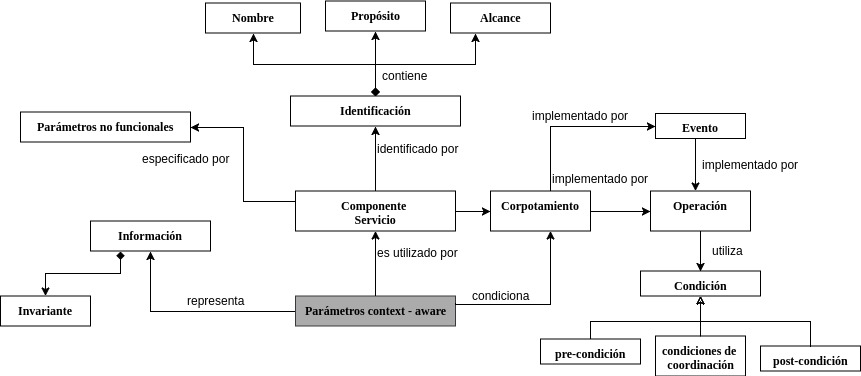
\includegraphics [width=6 in,totalheight=3 in]{Ch4/contrato_conceptual}
 % .: 0x0 pixel, 0dpi, 0.00x0.00 cm, bb=
\end{center}
\caption{Características del ContratoDHD}
\label{fig:contratov2}
\end{figure}

A continuación, se describen para cada componente sus principales características, roles y funciones que cumplen dentro del esquema conceptual general.

\begin{itemize}

\item \textit{Identificador}.

El \textit{Identificador} se utiliza para la identificación de una \textit{componente servicio} para un determinado contexto por un único nombre en un espacio de nombre.

\item \textit{Comportamiento.}

De acuerdo con los roles asignados en un determinado contexto, una \textit{Componente Servicio} expone sus  \textit{comportamientos} a través de \textit{operaciones} publicadas. Las operaciones pueden ser definidas en dos tipos – operaciones que ejecutan cómputos o transformaciones (tipo “update”) y operaciones que proveen algún tipo de información sobre consultas (tipo “query”). Estas se encuentran enteramente especificadas en base
a un contrato, con el uso de \textit{precondición}, \textit{post-condición} y \textit{condicionales} para lograr coordinación entre contratos. En las condiciones de coordinación se especifican cómo requerir y proveer operaciones, así como también los eventos publicados y recibidos son coordinados en los momentos adecuados. Para lograr una comunicación precisa con un componente servicio, no sólo se tiene en cuenta qué operación fue provista o requerida y cómo el ejecutor ha lanzado el evento apropiado, sino también, cómo todas esas actividades están mutuamente relacionadas para ser aprovechadas por el objeto consumidor. Un evento del contexto que lanza una operación dada, puede ser parte de un conjunto de precondición, mientras que un evento emitido a través de una exitosa operación puede ser parte de una postcondición.


Las operaciones provistas por la componente de servicio deben estar asociadas, a fin de determinar cuáles deben ser completadas antes de la activación de un servicio asociado. Este tipo de asociación es posible de efectuarse en forma paralela o ser sincronizado por otro camino mecanismo. Por ejemplo, la figura \ref{fig:contratov2} representa el caso de una componente de servicio denominado \textit{Manejador\_Orden}, la operación \textit{ejecutar\_orden()} no puede ser invocada hasta que el servicio que la consume no esté correctamente autorizado por el componente de servicio \textit{Administrador\_Registros}. Otro ejemplo, la operación \textit{borrar\_registro()} no puede ser invocada si la operación \textit{ejecutar\_orden()} con el mismo parámetro \textit{orden\_id} no fue previamente completada.


\begin{figure}
\begin{center}
 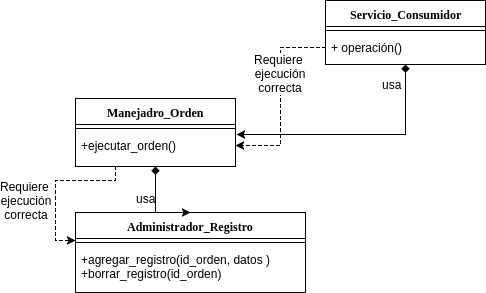
\includegraphics [width=3.5 in,totalheight=2 in]{Ch4/servicios_coordinados}
 % .: 0x0 pixel, 0dpi, 0.00x0.00 cm, bb=
\end{center}
\caption{Coordinación de servicios}
\label{fig:servicios_coordinados}
\end{figure}



\item \textit{Tipos de Información.}

Una componente de servicio debe manejar, usar, crear o tener cierta información de recursos con el propósito de proveer información y ejecutar acciones adecuadamente. El elemento \textbf{Tipos de Información} del contrato, como su nombre lo indica, define el tipo de información relevante para las componentes asociadas al contrato, así como también restricciones y reglas sobre instancias específicas para cada tipo. De esta manera, se representa un modelo de información lógica, en el sentido del cómputo, de una componente de servicio. Formalmente, esta información de tipos puede ser considerada como definiciones de tipos de los parámetros de las operaciones o tipos relacionados con ellos.

\item \textit{Configuración de Parámetros Context-Aware}

Un componente servicio depende del contexto de su actual entorno. La misma, para utilizarse en diferentes contextos, logrando la adaptación a eventuales cambios, debe tener definido un conjunto de parámetros de configuración. Ejemplos de estos parámetros pueden ser: Contexto-del-Usuario (CU) - en un sentido similar a lo definido en el capítulo anterior, locación en tiempo y espacio de los servicios consumidos y suministrados. Estos parámetros pueden ser enviados dentro de las invocaciones de las operaciones de los servicios o por medio de otros caminos, mediante componentes de servicios que pueden adaptar su comportamiento ante el cambio de contexto en una determinada situación.

La configuración de parámetros está directamente asociada a las relaciones de las operaciones de los servicios para lograr una mejor adaptación a la medida de las circunstancias brindada por la información relevada del contexto. El concepto de la configuración de los parámetros context-aware, es un paso muy importante hacia la concepción de servicios automatizados y autoadaptables (tomando el sentido paradigmático de los teóricos de la Inteligencia Artificial).


\item \textit{Parámetros no funcionales.} 

Un componente servicio puede definir un conjunto de los llamados parámetros no funcionales que caracterizan a la “calidad” de sus prestaciones dentro de un determinado contexto. Estos parámetros, son elementos para los consumidores delos servicios que permiten optar por el uso de un determinado servicio, o buscar otro con el mismo o similar contrato. Como ejemplo de parámetros no funcionales podemos mencionar: Performance, Fiabilidad, Tolerancia a Fallos, Costos, Prioridad y Seguridad.

\end{itemize}


\section{ContratosDHD: Contratos sensibles al contexto para el DHD}
\label{sec:estrategiasca}


Una vez más se abordará una definición teniendo en cuenta cuestiones tecnológica inherentes a su implementación. La implementación de los contratos para el DHD debe cumplir el diseño de la figura \ref{fig:contratov2} y se debe ajustar a la metodología del agregado del framework JCA\footnote{JCAF is designed to support Context-Aware Computing and has come out of our work with the design of context-aware applications in a hospital environment.} % (véase forma de agregado en la sección \ref{sec:subsistemas})
 

Para esta tesis se han explorado diferentes implementaciones de los contratos de Meyer \cite{Meyer}, referentemente aquellas que se puedan ajustar mejor en nuestros desarrollos y diseño. De esta manera, se tuvieron en cuenta avances donde el uso de contrato para la representación de aserciones permitan una buena integración para el DHD. 

Desafortunadamente, existen pocos lenguajes que soportan técnicas de aserciones (ej. Eiffel \footnote{Eiffel fue ideado en 1985 por Bertrand Meyer. Es un lenguaje de programación orientado a objetos centrado en la construcción de software robusto. Su sintaxis es parecida a la del lenguaje de programación Pascal. Una característica que lo distingue del resto de los lenguajes es que permite el diseño por contrato desde la base, con precondiciones, postcondiciones, invariantes y variantes de bucle, invariantes de clase y aserciones.}). Las forma de implementación y la tecnología (e.j., lengujes de programación, etc.) que se utiliza tienen una alta incidencia en el diseño y arquitectura. En este sentido, se analizaron tres diferentes tipos de estrategias de implementación.

\begin{itemize}

 \item \textbf{\textit{Built in}}: significa que el soporte de los contratos está incluido en los el lenguaje de programación. Donde se tienen constructores de lenguajes para la formulación de aserciones de diferentes formas. La corrección de la sintaxis de la aserción es directamente chequeada por el compilador. Además, el entorno de ejecución posibilita que se controle dicho chequeo en tiempo de ejecución. Las mayores ventajas de estas implementaciones tienen que ver con la homogénea integración de las aserciones dentro del lenguaje de programación, i.e., los mensajes de error son consistentes, las herramientas de depuración permiten un adecuado manejo e implementación de aserciones (ej., correctitud de número de línea y traza de ejecución).


\item \textbf{\textit{Preprocessing}}: Esta es la clase más popular de soporte para las aserciones en los lenguajes de programación. La idea general es la formulación de aserciones separadas del programa o incluirlas como comentarios. Utiliza un pre-proceso para entretejer aserciones entre el programa o transformar los comentarios en porciones de código que la ejecuten. La principal ventaja de este método es la separación entre el contrato y la lógica de programación.


\item \textbf{\textit{Metaprogramming}}: La metaprogramación refiere a "programación para los niveles de la interpretación de los programas, o en otras palabras, para extender las interpretaciones de un lenguaje de programación hacia una explicación específica"\cite{Temp1}.
Programas que tienen la posibilidad de razonar sobre si mismo tiene la propiedad llamada reflectiva (en inglés ``reflective capacity``). Por ejemplo, el lenguaje de programación Java tiene capacidades reflectivas y es implementada a través de una API. La mayor ventaja de la metaprogramación es que no es necesario el uso de preprocesamiento. No obstante, un entorno de ejecución especializado debe ser usado para el chequeo de las aserciones.
\end{itemize}

\subsection{Sistema que proveen soportes para el desarrollo de software basado en contratos} \label{sec:sistemasca}

Se analiza brevemente diferentes sistemas que proveen soporte para el desarrollo de software basado en contratos a través del lenguaje de programación Java. Estas propuestas fueron estudiadas basándose en los prototipos disponibles para evaluar el impacto en nuestra particular implementación, i.e., no solamente una evaluación teórica. No fueron consideradas propuestas que usan técnicas de algebraicas o lógica de alto orden. De la misma manera, sistemas como JML \cite{Leavens99} no fueron considerados. 

A continuación se detalla para cada propuesta de sistema el nombre, el tipo de resolución implementada (lenguajes de programación, extensiones de lenguajes, preprocesamiento, metaprogramación), consideraciones generales, características especiales y referencias.

\begin{itemize}

\item \textbf{Biscotti:}

\begin{itemize}
\item \underline{Tipo de soporte}: Extensión del lenguaje Java, tiene incorporado un soporte para compilación.
\item \underline{Información}: Biscotti se concentra en la implementación de especificaciones de comportamiento a través de interfases Java introduciendo palabras claves adicionales. 

\item \underline{Características especiales}: No es necesario hacer cambios para la máquina virtual java, esto es posible debido a que Biscotti usa reflección y facilita la creación de precondiciones, postcondiciones e invariantes visibles en tiempo de ejecución.

\item \underline{References}: \cite{Cicalese99}
\end{itemize}

Ejemplo: 

\begin{lstlisting}[language=Java]

        import biscotti.Biscotti;
        
        public class Main {
            public static void main(String[] args) {
                Biscotti biscotti = new Biscotti();
                String message = biscotti.bake("Hello, world!");
                System.out.println(message);
            }
        }
\end{lstlisting}



\item \textbf{Assertion Facility (JAF):}

\begin{itemize}
\item \underline{Tipo de soporte}: Implementado desde la versión 1.4 de Java. \item \underline{Información}: Desde la versión 1.4 de Java se incorporó palabra claves para aserciones para indicarles al compilador donde se encuentran las aserciones y su interpretación a través de la máquina virtual. Java solo soporta mecanismos de aserciones simples que permiten instrumentar condiciones a través de métodos. \item \underline{Características especiales}: El chequeo de las aserciones pueden ser fácilmente habilitadas y deshabilitada y los rastros de las aserciones pueden ser completamente eliminados de los archivos de las clases. \item underline{Referencias}:\cite{Sun02,Rogers01a,Rogers01b}.
\end{itemize}

Ejemplo: 

\begin{lstlisting}[language=Java]
import 
...

public class Main {
    public static void main(String[] args) throws Exception {
        Session session = Session.getDefaultInstance(System.getProperties());
        MimeMessage message = new MimeMessage(session);
        message.setFrom(new InternetAddress("sender@example.com"));
        message.setRecipient(Message.RecipientType.TO, new InternetAddress("recipient@example.com"));
        message.setSubject("Test message with attachment");

        MimeBodyPart textPart = new MimeBodyPart();
        textPart.setText("Hello, world!");

        MimeBodyPart attachmentPart = new MimeBodyPart();
        FileDataSource fileDataSource = new FileDataSource("file.txt");
        DataHandler dataHandler = new DataHandler(fileDataSource);
        attachmentPart.setDataHandler(dataHandler);
        attachmentPart.setFileName(fileDataSource.getName());

        MimeMultipart multipart = new MimeMultipart();
        multipart.addBodyPart(textPart);
        multipart.addBodyPart(attachmentPart);

        message.setContent(multipart);

        Transport.send(message);
    }
}
\end{lstlisting}



\textbf{\item ContractJava:}
\begin{itemize}
    \item \underline{Tipo de soporte}: ContractJava es el típico preprocesamiento en el que se
    genera código Java. 
    
    \item \underline{Información}: El preprocesamento soporta los usuales tipos de precondiciones, postcondiciones y aserciones. 
    
    \item \underline{Características especiales}: Soporta comportamiento de
    subtipo (Behavioral subtyping)\cite{subtyping}  
    
    \item \underline{Referencias}: \cite{Findler01}
    
\end{itemize}

\begin{lstlisting}[language=Java]
import contractjava.Contract;

public class Main {
    public static void main(String[] args) {
        Contract contract = new Contract();
        contract.requires(args.length > 0, "At least one argument is required");
        contract.ensures(args[0].equals("Hello"), "The first argument must be 'Hello'");
        System.out.println(args[0]);
    }
}
\end{lstlisting}



\textbf{\item iContract:}
\begin{itemize}
    \item \underline{Tipo de soporte}: Preprocesamiento en el que se genera código Java para ser compilado por el compilador estándar Java.
    \item \underline{Información}: Las aserciones son escritas como documentación de métodos y clases 
    \item \underline{Características especiales}: iContract soporta operaciones sobre colecciones y provee herramienta adicionales para la documentación de aserciones en Java Doc (iDoclet) y para facilitar el rediseño de clases Java (iDarvin)
    \item \underline{Referencias}: \cite{Kramer98,Enseling01}
\end{itemize}


\begin{lstlisting}[language=Java]
import icontract.Contract;
    
public class Main {
    @Contract("requires args.length > 0; ensures args[0].equals('Hello');")
    public static void main(String[] args) {
        System.out.println(args[0]);
    }
}
\end{lstlisting}


\textbf{\item Jass:}
\begin{itemize}
    \item \underline{Tipo de soporte}: Preprocesador para la generación de código Java  antes de la copilación.
    \item \underline{Información}: Los significados de las aserciones son especificados por medio de comentarios para métodos y clases. Un programa Jass es un programa Java bien formado y puede ser transformado directamente para el compilador estándar Java.
    \item \underline{Características especiales}: Jass soporta cuantificadores universales y existenciales para conjuntos finitos. 
    \item \underline{Referencias}: \cite{Bartezko01}
\end{itemize}


\begin{lstlisting}[language=Java]
import jass.Assert;

public class Main {
    public static void main(String[] args) {
        Assert.assertTrue(args.length > 0, "At least one argument is required");
        Assert.assertEquals(args[0], "Hello", "The first argument must be 'Hello'");
        System.out.println(args[0]);
    }
}
\end{lstlisting}


\textbf{\item Jcontract:}
\begin{itemize}

    \item \underline{Tipo de soporte}: Preprocesador para la generación de código
    java para el compilador estándar Java.
    
    \item \underline{Información}: Las aserciones se especifican como comentarios para
    métodos y clases.
    
    \item \underline{Características especiales}: Jcontract soporta cuantificadores     existenciales y universales para tipos de los colecciones. Además, Jcontract está estrechamente integrado con la herramienta Jtest\cite{Parasoft02a}. Jtest la información de especificación contenida en el contrato, luego crea una
    clase de test ejecutable que permite testear si se cumple la funcionalidad de la clase especificada. Incluye herramienta de generación de javadoc para la generación de documentación API donde contiene las 
    specificaciones de las aserciones. 
    
    \item \underline{Referencias}:\cite{Parasoft02b}

\end{itemize}

\begin{lstlisting}[language=Java]
import org.jcontract.Contract;

public class Main {
    @Contract(precondition = "args.length > 0", postcondition = "result.equals('Hello')")
    public static String getFirstArgument(String[] args) {
        return args[0];
    }

    public static void main(String[] args) {
        System.out.println(getFirstArgument(args));
    }
}
\end{lstlisting}


\textbf{\item Handshake:}
\begin{itemize}
    \item \underline{Tipo de soporte}: Provee aserciones a través de reflección (Javareflection). 
    \item \underline{Información}: Los contratos son separados en archivos diferentes. Las clases son combinadas en tiempo de ejecución combinando dinámicamente los archivos de los contratos y las clases Java. \item \underline{Características especiales}: Debido a las propiedades dinámicas los contratos son incorporados a las clases a nivel de código de ejecución.
    \item \underline{Referencias}:\cite{Duncan98}
\end{itemize}

\begin{lstlisting}[language=Java]
import handshake.Handshake;

public class Main {
    public static void main(String[] args) {
        Handshake handshake = new Handshake();
        String message = handshake.greet("Hello, world!");
        System.out.println(message);
    }
}
\end{lstlisting}

\textbf{\item jContractor:}
\begin{itemize}
    \item \underline{Tipo de soporte}: jContractor se basa puramente en librerías
    base
    utilizando metaniveles de información deducidas de los archivos de las clases
    Java y usa la ejecución dinámica de las clases Java a través de la
    interpretación de cambios reflectivos en tiempo de ejecución. 
    \item \underline{Información}: La codificación del contrato (precondiciones,
    postcondiciones e invanriantes) son incorporados a las clases por medios del
    especificados con determinadas convenciones de nombres.
    \item \underline{Características especiales}: Dentro de las postcondiciones de
    un método
    es posible controlar los resultados esperados con otros resultados específicos.
    \item \underline{Referencias}:\cite{Parasoft02b} 
\end{itemize}
    
\begin{lstlisting}[language=Java]
import jcontractor.Contract;
public class Main {
    @Contract("requires args.length > 0; ensures result.equals('Hello');")
    public static String getFirstArgument(String[] args) {
        return args[0];
    }

    public static void main(String[] args) {
        System.out.println(getFirstArgument(args));
    }
}
\end{lstlisting}


%\colorbox{yellow}{*** conectar esto ***}

Teniendo en cuenta la característica del modelo conceptual de contrato de la figura \ref{fig:contratov2} y de las infraestructuras utilizadas para su implementación, se comienza a determinar las primeras consideraciones a tener en cuenta en el diseño de contratos sensibles al contexto para el DHD.

\begin{defi} [ContratoDHD]

El ContratosDHD es una infraestructura para la aplicación del concepto de Diseño por Contrato (DbC) de Bertran Meyer (2002). El DbC es una técnica diseñada por Meyer y característica central de su lenguaje de programación Eiffel\cite{Meyer}. El DbC se utiliza con cualquier lenguaje de programación, para validar que el software cumpla con su especificación (contrato). El contrato establece condiciones de uso e implementación denominadas aseveraciones que componentes de software con un rol de "clientes" y otras de "proveedores" deben cumplir. En el DbC se utilizan tres tipos de aseveraciones: \underline{Precondición:} restricciones bajo las cuales una rutina funcionará correctamente.  \underline{Postcondición:} describe el efecto de la rutina. \underline{Invariante de clase:} restricciones que deben satisfacerse por cada objeto tras la ejecución de los métodos y constructores. 
Para la instrumentación de ContratosDHD se crearon dos tipos de componentes esenciales que permitan una correcta integración, a niveles de diseño e implementación, con una plataforma e-learning:

\begin{itemize} \label{CEC}

 \item Componente esencial tipo \#1: Componentes del contrato para la implementación de las
propiedades de sensibilidad al contexto. Los elementos que integran este
subsistema son:
 
      \begin{itemize}
       \item Arquitectura para la adaptación del contexto
       \item Funcionalidades 
      \end{itemize}
      
  \item Componente esencial tipo \#2: Componentes de conexión e implementación de un patrón de
diseño que permite la coordinación de contratos.
	    \begin{itemize}
	    \item Reglas de coordinación
		  
		  \begin{itemize}
		   \item Condicionales especiales
		   \item Condicionales comunes 
		  \end{itemize}
	    \item Componentes de conexión
	    \end{itemize}
\end{itemize}
\end{defi} 



\subsection{Componentes esenciales de los contratos sensibles al contexto}

En este apartado se exponen diferentes tipos de componentes, denominados como \textbf{componentes esenciales}, para capturar datos de contexto. Estos datos serán representados en un modelos abstracto de información  utilizado para adaptar los servicios, de una aplicación, a los usuarios o artefactos de software que lo utilizan; en función de sus propios estados o estado del entorno. Para este propósito, se parte del modelo propuesto por A. Dey (2000) en su tesis doctoral \cite{Dey} donde se propone una arquitectura conceptual para los sistemas sensibles  al contexto. A continuación, se enumeran las principales características de los elementos que definen esa arquitectura:


\begin{itemize}

\item \textbf {Servidor de contexto:} Permite el acceso de múltiples clientes a los datos de forma remota.  Libera a los clientes de recursos que demandan operaciones intensivas.  Debe considerar el uso de protocolos apropiados para la representación de las variantes de información de contexto, rendimiento de la red, calidad de los parámetros de los servicios.


\item \textbf{Widgets}:  Encapsulamiento.  Intercambiable.
Controlado a través de un manejador de widget. En el caso que las
componentes estén acopladas incrementan la eficiencia al costo de perder robustez ante fallas de componentes.


\item \textbf{Networked services:}  Similar a la arquitectura
servidor de contexto. (modelo orientado a objeto).  tiene la eficiencia de la arquitectura \textbf{widget} debido a la complejidad de las componentes bases de red, pero provee robustez.


\item \textbf{Blackboard model:}  Procesos post-mensajes para
compartir medios, pizarrón (modelo basado en datos). Simplicidad en el agregado de nuevos recursos de contexto.  Fácil configuración.  Un servicio centralizado.  Carece de eficiencia en la comunicación (son
necesarios dos puntos de conexión por comunicación)

\end{itemize}

La componente \textit{Widget} cumple un importante papel en la propuesta de Dey. Un \textit{widget} es un componente de software que brinda una interfaz pública para algún tipo determinado de sensores (hardware) (Dey, A. K. y G. D. Abowd, 2000). Los \textit{widgets} encapsula detalles de datos censado a nivel de hardware. También, son componentes con alto grado de reusabilidad facilitando las tareas de diseño e implementación de aplicaciones en las que se utiliza información de contexto capturadas por sensores. El encapsulamiento en los \textit{widgets} permite intercambiarlos entre aquellos que proveen el mismo tipo de datos; por ejemplo, intercambiar un \textit{widget} de radiofrecuencia por un \textit{widget} de una cámara filmadora donde ambos recolectan datos de locación de individuos).

Usualmente los \textit{widgets} son controlados por módulos de administrador de \textit{widget}. Una buena práctica para administrar \textit{widgets} es combinar sus funcionamientos de forma acoplada para incrementar su eficiencia, aunque esta decisión hace perder robustez ante fallas en componentes.

A continuación, se presentan cinco categorías de componentes agregadas a las anteriores para el manejo del contexto.


\begin{itemize}


 \item \textbf{Context Widgets:} se encarga de la adquisición de información de contexto; 

\item \textbf{Interpreters:} cumplen la función de transformar y aumentar el grado de abstracción de la información de contexto, deben combinar varias piezas de contexto para producir información procesada de alto nivel;


\item \textbf{Aggregator:} es un componente que junta información de contexto de una entidad del mundo real, tales como información sobre datos de usuarios, locación, etc. Actúa como un textit{getway} entre las aplicaciones y  widgets, ocultando aún más la complejidad de los mecanismos de adquisición de contexto. En otras palabras, el \textbf{aggregator} transforma la información adquirida por los sensores, siguiendo una serie de reglas de transformación predetermindas para los propósitos adecuados.


\item \textbf{Services:} brindan servicios en un determinado ambiente
adaptando su funcionalidad al tipo de información de contexto adquirida; 

\item \textbf{Discoveres:} permite que las aplicaciones (y otras entidades)
optimicen su desempeño pudiendo determinar la característica del entorno
(tipo de restricciones y dominio de aplicación). Entre estos componentes
se pueden establecer un número limitado de relaciones.

\end{itemize}

Los widgets son consultados y/o notificados ante eventuales cambios en los de información del estado del cliente. Los clientes pueden ser\textit{aplicaciones}, \textit{aggregators} u otros \textit{widgets}. A su vez, \textit{aggregators} actúa como un puente entre \textit{widgets} y aplicaciones. Un \textit{interpreters} puede ser solicitado en un determinado estado por un \textit{widget}, \textit{aggregator} o \textit{aplicaciones}. Los \textit{services} son lanzados por las aplicaciones (también otros componentes pueden hacer uso de los servicios). \textit{Discoveres} se comunica con todos los componentes, se adquiere desde los \textit{widget}, \textit{interpreters} y \textit{aggregators}, y provee información a las aplicaciones por medio de notificaciones y consultas.

La figura \ref{fig:toolkit} expone una posible configuración con dos dispositivos de censado, dos \textit{widgets}, un \textit{aggregator}, dos \textit{interpreters}, un \textit{servicio}, un \textit{discoverer} y dos \textit{aplicaciones}.


\begin{figure}
\begin{center}
 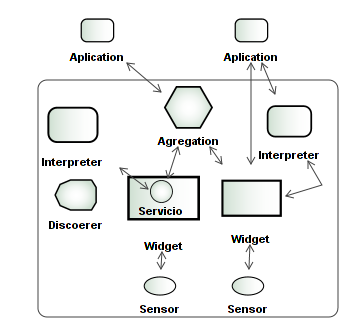
\includegraphics [width=5 in,totalheight=2 in]{Ch4/ContextToolsKit.png}
\caption{Elementos para la toma de contexto en los ContratosDHD}
\label{fig:toolkit}
 % .: 0x0 pixel, 0dpi, 0.00x0.00 cm, bb=
\end{center}
\end{figure}


En el instante en que algún componente contexto se encuentre disponible, registra sus capacidades en un \textit{discoverer}. Esto permite que los \textit{aggregators} encuentren \textit{widgets} e \textit{interpreters}. De la misma manera, las aplicaciones se relacionan con los \textit{aggregators}, \textit{widget} e \textit{interpreters}. Un sensor provee datos para que un \textit{context widget} encarga de almacenarlo como información contexto. La aplicación puede llamar a un \textit{interpreter} para obtener un mayor nivel de abstracción de los datos y luego pone el contexto a disposición para que pueda ser accedido por otros componentes y aplicaciones.

Un \textit{aggregator} recolecta información de contexto de las entidades, representadas por los \textit{widgets}. Finalmente, las aplicaciones pueden consultar o suscribirse a los \textit{agreegators} (o directamente con los \textit{widgets}, si se quiere). También es posible, llamar a \textit{interpreters}, si se requiere otro nivel de representación de la información de contexto diferente a las que proveen los \textit{widgets} y \textit{aggregators}).

Estos componentes se ejecutan independientemente de las aplicaciones, asegurando una continua adquisición de información de contexto y el uso de múltiples aplicaciones. Además, todos los componentes y aplicaciones se comunican entre ellos automáticamente usando protocolos y lenguajes conocidos.

Esto da lugar a que los programadores que implementan un particular componente o aplicación puedan comunicarse con otro componente sin tener conocimiento de los mecanismos usados para lograr la interacción.

\parskip=1cm 

\subsection{Una implementación del subsistema para CEC\#1}

La implementación del subsistema de las componentes esenciales para el agregado de propiedades de sensibilidad al contexto (CEC\#1) tienen dos significancia para esta tesis. En primer lugar, es brindar un ejemplo concreto de intregración utilizando parte del recorrido teórico y documental de tipos de sistemas (secciones \ref{sec:sistemasca})  y estrategias (secciones \ref{sec:estrategiasca}). En segundo lugar, presentar nuevos conceptos y definiciones que permitan generalizar este tipo de propuestas de comunicación entre sistemas. 

Para este caso se utiliza como subsistema para CEC\#1 el framework JCAF  (\textit{Java Context-Awareness Framework}). A través de JCAF se implementan la ejecución de servicios (servicios de herramientas colaborativas) por medio de la infraestructura orientada a servicios basada en la idea de la división de la adquisición de contexto, su manejo y  distribución o conexión con los \hyperref[contratosDHD]{ContratosDHD}. Además JCAF provee un modelo de programación para Java extensible, genérico y expresivo orientado al desarrollo e implementación de aplicaciones sensibles al contexto y modelado de contexto. En la  publicación \cite{JCAF} se brindan más detalles sobre cómo JCAF difiere de otros soporte middleware para aplicaciones sensibles al contexto. 


Para describir más apropiadamente la participación que JCAF tiene para nuestra propuesta de implementación es necesario determinar cu´ales de los aspectos orientados a servicios serán recogidos. De esta manera se brinda una dedición sobre el contexto en el que se tienen en cuenta los servicios.


\begin{defi}[ServiciosDHD:] \label{serviciosDHD}

Se denomina \textbf{servicioDHD} a cualquier implementación sobre las funcionalidades de una herramienta, de un espacio colaborativo, (1) que tenga interfases de comunicación con la componente parámetros Context-Aware (figura \ref{fig:contratosv2}) y  (2) que su implementación contenga elementos que representan entidades participantes e información de contexto \cite{Dey}. En otras palabras, la implementación de un \textbf{servicioDHD} está compuesta por módulos para la representación y uso de contexto, y que los mecanismos de ejecución estén mediados por los \hyperref[contratosdhd]{ContratosDHD} 

\end{defi}

\subsubsection{Infraestructura para serviciosDHD}

A partir de la infraestructura que brinda JCAF para combinar modelos e implementaciones de servicios con información de contexto, se realizarán adaptaciones que permitan incorporar al contrato sensible al contexto como una nueva pieza de software. De esta manera se creará una nueva infraestructura de servicios denominada \hyperref[serviciosDHD]{serviciosDHD}. Con esta adaptación, desde la perspectiva del usuario, los servicios de la aplicación se adaptarán a su contexto. 

\colorbox{green}{La parte mas importante. Sacar este comentario}


% todo: rehacer este gráfico
\begin{figure}
\begin{center}
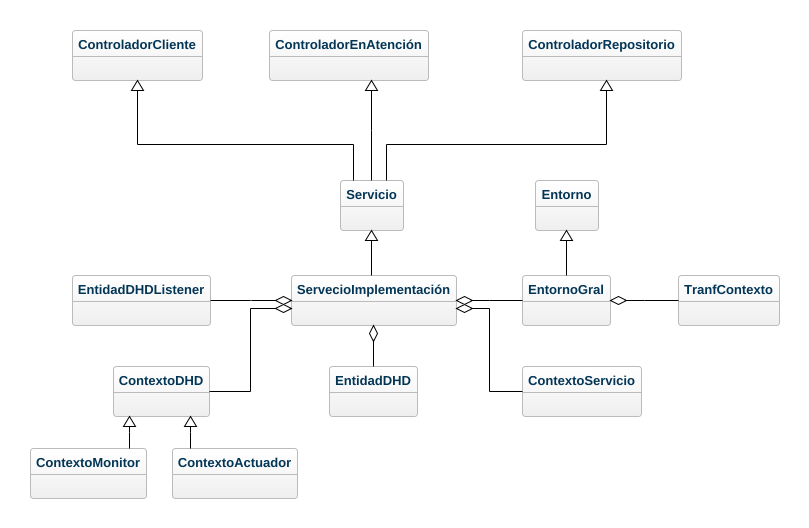
\includegraphics[width=5 in,totalheight=3.2 in]{Ch4/serviciosDHD.png}
% .: 0x0 pixel, 0dpi, 0.00x0.00 cm, bb=
\caption{Arquitectura de ejecución de serviciosDHD}
\label{fig:serviciosDHD}
\end{center}
\end{figure}


\subsection{Coordinación de los contratos sensibles al contexto}

%Elementos de la componente contrato 
El contrato es la información de las expectativas y responsabilidades de un componente. El contrato puede ser configurado por medio de diferentes mecanismos, desde el lenguaje coloquial hasta un lenguaje de especificación formal. Por ejemplo, el uso de un lenguaje basado en XML para los casos en que sean necesarias especificaciones que puedan ser procesadas por máquinas. 


\begin{lstlisting}[language=XML]
    
<Contract>
  <Inputs>
    <Input name="x" type="float" />
    <Input name="y" type="float" />
  </Inputs>

  <Outputs>
    <Output name="result" type="float" />
  </Outputs>
  
  <Behaviors>
    <Behavior name="Preconditions">
      <Condition>
        <Expression>
            <![CDATA[x > 0]]>
        </Expression>
        <ErrorMessage>
            <![CDATA[x must be greater than 0]]>
        </ErrorMessage>
      </Condition>
      
      <Condition>
        <Expression>
            <![CDATA[y > 0]]>
        </Expression>
        <ErrorMessage>
            <![CDATA[y must be greater than 0]]>
        </ErrorMessage>
      </Condition> 
    </Behavior>
  
    <Behavior name="Postconditions">
      <Condition>
        <Expression>
            <![CDATA[result > 0]]>
        </Expression>
        <ErrorMessage>
            <![CDATA[result must be greater than 0]]>
        </ErrorMessage>
      </Condition>
    </Behavior>
  </Behaviors>
</Contract>

\end{lstlisting}



En este caso, el contrato especifica que el componente espera dos entradas de tipo \textit{float} llamadas "x" \\e "y", y que producirá una salida de tipo \textit{float} llamada "result". Además, se especifican dos precondiciones que deben cumplirse antes de llamar al componente: "x" \\y "y" deben ser mayores que cero. También se especifica una postcondición que se debe cumplir después de que el componente haya terminado de ejecutarse: la salida "result" debe ser mayor que cero.


El tipo de tecnología y forma de implementación de los contratos es transparente para los objetos que consumen los servicios en donde se encuentran involucrados. La configuración de un elemento contrato que forma parte de las componentes de un servicio representa la información necesaria del mismo para ser utilizado por el invocador, sin necesidad de que el objeto invocador tenga detalles de la ejecución.

El contrato representa una enriquecida y efectiva interfaz de construcción con acceso a información sobre las componentes de los servicios y datos del contexto representados en la figura \ref{fig:serviciosDHD}, con el propósito de 


En este caso, el concepto de interfaz tiene mayor significación que un simple acceso a un contrato de reglas entre una  componente proveedora de servicio y su correspondiente componente cliente o consumidor.

En la figura 2 podemos observar los elementos conceptuales básicos de esta componente a través de una serie de elementos en relación con el contrato. Este metamodelo tiene las características conceptuales y operativas que se fundamentan en “Obra abierta”.

Para una mejor comprensión de las componentes del modelo explicitaremos
a continuación su caracterización y funciones particulares.

\textbf{Identificador}: una componente servicio es identificada para un
determinado
contexto por un único nombre en el espacio de identificación.

\textbf{Comportamiento}: de acuerdo con los roles asignados en un determinado
contexto, una componente servicio expone comportamientos correspondientes a
provisión y pedido de operaciones, y/o publicaciones y recepción desde/hacia
cada contexto. Las operaciones pueden ser definidas de dos tipos: operaciones
que ejecutan cómputo o transformaciones (tipo update) y operaciones que proveen
algún tipo de información sobre consultas (tipo query). Éstas se encuentran
enteramente especificadas en base a un contrato, con el uso de precondición,
poscondición y condicionales para lograr la coordinación entre contratos. En las
condiciones de coordinación se especifican cómo requerir y proveer operaciones,
así como también los eventos publicados y recibidos son coordinados en los
momentos adecuados. Para lograr una comunicación precisa con una componente
servicio, no sólo se tiene en cuenta qué operación fue provista o requerida
y cómo el ejecutor ha lanzado el evento apropiado, sino también cómo todas
esas actividades están mutuamente relacionadas para ser aprovechadas por el
objeto consumidor. Un evento del contexto que lanza una operación dada
puede ser parte de un conjunto de precondición, mientras que un evento emitido
a través de una exitosa operación puede ser parte de una poscondición.


Las operaciones provistas y requeridas por la componente de servicio
deben estar asociadas, a fin de determinar las operaciones que deben ser completadas
antes de la activación de un servicio (qué es posible ejecutar en paralelo
o ser sincronizado por otro camino). Por ejemplo, en el caso de una
componente de servicio ManejadorOrden, la operación HacerOrden no puede
ser invocada hasta que el servicio que la consume no esté correctamente autorizado
por el componente de servicio AdministradorRegistros, o la operación
DeleteOrder no puede ser invocada si la operación HacerOrden con el mismo
parámetro OrdenID no fue previamente completada.
Tipos de información: una componente de servicio debe manejar, usar, crear o
tener cierta información de recursos con el propósito de proveer servicios adecuadamente.
Este elemento del contrato define el tipo de información relevante
para las componentes asociadas al contrato, así como también
restricciones y reglas sobre instancias de esos tipos. Esto representa un modelo
de información lógica de una componente de servicio. Formalmente, esta
información de tipos puede ser considerada como definiciones de tipos de los
parámetros de las operaciones o tipos relacionados a ellos.
Configuración de parámetros context-aware: una componente servicio depende
del contexto de su actual entorno. La misma, para utilizarse en diferentes contextos
logrando la adaptación a eventuales cambios, debe tener definido un
conjunto de parámetros de configuración. Ejemplos de estos parámetros pueden
ser: Contexto del Usuario (CU), en un sentido similar a lo definido en el
capítulo anterior, locación en tiempo y espacio de los servicios consumidos y
suministrados. Estos parámetros pueden ser enviados dentro de las invocaciones
de las operaciones de los servicios o por medio de otros caminos, mediante
componentes de servicios que pueden adaptar su comportamiento ante el
cambio de contexto en una determinada situación.
La configuración de parámetros está directamente asociada a las relaciones
de las operaciones de los servicios para lograr una mejor adaptación a la
medida de las circunstancias brindada por la información relevada del contexto.
El concepto de la configuración de los parámetros context-aware es un
paso muy importante hacia la concepción de servicios automatizados y autoadaptables
(tomando el sentido paradigmático de los teóricos de la inteligencia
artificial).

\textbf{Parámetros no funcionales:} una componente servicio puede definir un
conjunto de los llamados parámetros no funcionales que caracterizan la “calidad”
de sus prestaciones dentro de un determinado contexto. Estos parámetros
son elementos para los consumidores de los servicios que permiten optar por el
uso de un determinado servicio, o buscar otro con el mismo o similar contrato.
Como ejemplo de parámetros no funcionales podemos mencionar: performance,
fiabilidad, tolerancia a fallos, costos, prioridad y seguridad.


\subsubsection {Coordinación}

En términos generales, la coordinación de contratos es una conexión establecida
entre un grupo de objetos (en nuestras consideraciones los participantes
serían un objeto cliente y un determinado servicio), donde reglas, normas y
restricciones (RNR) son superpuestas entre los actores participantes, estableciendo
con un determinado grado de control las formas de interrelación (o
interacción).

El tipo de interacciones establecidas entre las partes es más satisfactoria
que las que se pueden lograr con UML o lenguajes similares (orientados a objetos)
debido a que éstas contienen un mecanismo de superposición donde se
toman como argumento los contextos. Cuando un objeto cliente efectúa una
llamada a un objeto suministro, el contrato “intercepta” la llamada y establece
una nueva relación teniendo en cuenta el contexto del objeto cliente, el
del objeto servidor e información relevante (respecto de la relación) adquirida
y representada como contexto del entorno. Como condición necesaria, la
implementación de los contratos no debe alterar el diseño y funcionalidad en
la implementación de los objetos.


\textcolor{red}{completar}



\section{Condicionales especiales para las reglas de los contratos}

% todo: definir obra abierta

La posibilidad de incorporar contratos sensibles al contexto en los servicios de las herramientas de una plataforma e-learning, pone en relevancia la importancia de las reglas de los contratos. En cierta medida, las reglas representarán gran parte de la lógica de negocio de las propiedades nuevas de adaptación que obtendrán los servicios originales de las plataformas. De esta manera, los condicionales de esas reglas constituyen un componente principal a tener en cuenta en las decisiones de diseño e implementación.

Para un mejor entendimiento de este concepto se describe, a partir de un caso de uso concreto, características y relaciones que se producen en un ambiente e-learning al utilizar una determinada herramienta, que as sus vez, contiene servicios con conexiones a contratos, provisto con sus correspondientes reglas, en las que aparecen condicionales.  


En las implementaciones de campo de cursos de nivel superior realizadas por
el equipo de “Obra abierta”, uno de los recursos primarios que los educadores
utilizaban era el recurso registro de actividades de la plataforma e-learning; por lo general, este recurso es administrado con una herramienta denominada ''Registro de Actividades``.  La información que provienen de estos recursos será considerar como información de contexto perteneciente al entorno, y valores cuantitativo que resignifiquen una característica del comportamiento de un usuario, tal como se expuso en el trabajo \ref{paper_de_condicionales} 


Consultar los registros de actividades es una gesto muy usual para obtener
información sobre el “grado” de interactividad que los usuarios \cite{arqDHD3} tienen, basadas en las definiciones de interacción del concepto de Dispositivo Hipermedial. En los casos más básicos, existe una estructura tipo “planilla” (filas y columnas) en las que se detallan los registros con los siguientes campos: fecha, hora, usuario, tareas realizadas. Las tareas pueden estar significadas con valores explícitos como: “visitas al foro”, “visualización de perfiles de usuarios”, “obtención de recursos”, “modificación datos de la wiki”, etcétera.

Ahora se tomará como referencia de ejemplo un trabajo de campo realizado bajo la dirección de la Dra. Patricia San Martín. Para este caso, se tomó la información extraídas de los registros de actividades de un ambiente e-learning (“grado” de interactividad), como información de contexto. Esta metodología se aplicó específicamente durante una experiencia de taller, expuesta en el capítulo IV de \cite{DHD} bajo el título “Un diseño de taller físico-virtual-interactivo-comunicacional”.

En base a esta estrategia, se propone usar la información de interactividad como parámetro ''context-awareness'' de los contratos según lo referido en “Elementos de la componente contrato”, de ese mismo capítulo, podremos establecer un lazo de retroalimentación entre las prácticas efectuadas, por usuarios y la adaptación de los servicios de las herramientas. En este experiencia, se utilizó un ambiente e-learning de Moodle \cite{Moodle}, la información de las actividades de los usuarios fué administrada por la herramienta denominada ``Registro de Actividades de Moodle''. De esta manera, el lazo de retroalimentación mencionado se produce por la ejecución automáticas de los comandos ejecutados a través de los servicios, debido a la intervención de los contratos. Concretamente, este proceso ocurre cuando un servicio es invocado a través de una herramienta y ejecutada por un usuario. Este usuario tiene asociada una información de contexto determinada a través de los datos obtenidos del registro de actividades. En esta secuencia, interviene el contrato para decir cuales son las acciones que se deben efectuar. Esta decisión se toma en función de las reglas que configuran el contrato; aquí es donde intervienen los condicionales de las reglas, dependiendo los valores de verdad en cada instancia de evaluación. Ahora bien, si esos valores depende de la información de contexto, entonces deberán ser calculada con un mecanismo especializado para este propósito. En esta sección utilizaremos un modelo particular de métrica que permita calcular los valores de verdad de los condicionales, y una propuesta de integración de un mecanismo que se acople al modelo al framework del dispositivo hipermedial dinámico a través de los contratos sensibles al contexto.


\subsection{MCondicionales}


Ahora se clasificarán los condicionales dependiendo de la métrica de cálculo de sus valores de verdad. Para un mejor entendimiento, se sigue con la idea de aplicación de los requerimientos y objetivos anteriores. En primer lugar contamos con un ambiente e-learning de la aplicación Sakai con el agregado de la componente contrato sensible al contexto. En este caso, se toma como referencia la herramienta foro de Sakai, con las configuraciones e infraestructura definidas en la sección \ref{sec:arqDHD}. El framework que instrumenta Sakai, desde el punto de vista tecnológico, contiene los mismos conceptos que Moodle, con lo cual es posible continuar con el ejemplo de la información de contexto obtenida del registro de actividades. 


Continuamos con la descripción de los elementos e información necesaria para el diseño de los mecanismos de métrica que fueron usado como parte esencial de las reglas de los contratos, tomando como referencia un modelo de estandarización bien definido. Particularmente, la métrica formará parte del condicional de las reglas del contrato. A estos tipos de condicionales los denominaremos textbf{Mcondicional}. Conceptualmente no existe diferencia entre un Mcondicional y una condición común, los valores de verdad de ambos pueden depender de la invocación de métodos o funciones programadas para el sistema y colaborarán en la articulación de la ejecución de acciones (servicios y procesos computacionales). 

Al incorporar el concepto de métricas en contratos sensibles al contexto asociados a una herramienta de Sakai, concede que el sistema sea más adaptable a nuevos cambios del contexto de usuario. Si nos focalizamos en las interacciones de la herramienta Foro \footnote{La herramienta Foro de Sakai es un módulo de la aplicación diseñada para que un usuario instructor, o líder de un espacio e-learning, pueda crear espacios de discusión organizado con posibilidad de integrar contenidos de otras herramientas del mismo espacio. Es obligatorio mantener un orden basados en tópicos y categorías. Las intervenciones de los usuarios ocurren en formatos de hilos conversacionales a través publicaciones tipo post. Las conversaciones pueden ser creadas por usuarios estudiantes y moderadas por usuarios docentes.} de Sakai dentro de la complejidad de un proceso didáctico del estilo \hyperref[ProdA]{(ProdA)} (o investigativos y/o productivos), es posible que no siempre se puedan definir reglas de contratos para satisfacer propiedades de adaptación. Por lo tanto, el diseño y concepción de las reglas estarán singularizadas en función de la dinámica del proceso ProdA, debiendo ser explícitas y de clara implementación y por sobre todo, adaptables para los contextos específicos de los usuarios (en este caso de estudio, estudiantes a nivel de grado).


El primer paso es lograr la explicitación de las reglas del contrato y que los condicionales representen criterios de decisiones sobre aspectos relevantes del proceso didáctico (investigativo o productivo). Por ejemplo, un estudiante puede adquirir un servicio determinado de una herramienta, previo a la evaluación de una condición representada como condicional de una regla del contrato. En general, a estas reglas deben ser diseñadas con el cuidado de no incorporar
redundancias, ambigüedades o incoherencias, tanto entre las propias reglas de un contrato como con otras reglas implícitas inherentes de los servicios relacionados. De esta manera, definimos las reglas del contrato como un conjunto de condiciones, acciones y prioridades.

Para una mejor interpretación de como está conformadas las reglas, se establece una caracterización gramatical para identificar a los elementos que la componen:

\begin{center}
 

\begin{figure}


Una regla es una relación entre condicionales y acciones del estilo \Re: \mathbb{C} \rightarrow \mathbb{A}. 

\mathbb{C} es el conjunto de todos los posibles condicionales. 
\mathbb{A} es el el conjunto de todas las posibles acciones que se pueden  invocar desde un contrato. 

Las acciones 

dsdss
R:

\label{fig:representación_reglas}
\end{figure}


\end{center}


La condición es un expresión Boolean sobre relaciones (mayor, menor,
igual, distinto, etc.) entre parámetros y valores concretos.
Las acciones conforman un conjunto de asignaciones de valor a otros parámetros
también definidos por el tipo de regla. Algunos de los parámetros de
las acciones deben ser “métodos de cálculo” que permitan cambios en el comportamiento
de los servicios en los cuales estas reglas son aplicadas.
La prioridad permite simplificar la cantidad de reglas que se deben escribir:
en lugar de la escritura de una regla para cada combinación de posibilidades
de los valores de los parámetros, se asegura que dos reglas no puedan ser
ejecutadas simultáneamente. El usuario podría escribir una prioridad baja para
todas las reglas y luego, con prioridades altas, ir identificando las excepciones
para el caso configurado inicialmente.

En síntesis, las reglas son ejecutadas mediante un orden de prioridades. En
consecuencia, en cada tipo de regla, cada una tiene sólo una prioridad.
Para ejemplificar este concepto, consideremos una regla donde, dependiendo
del tipo y cantidad de interacciones de un sujeto en formación (por
ejemplo, Juan Pérez), el servicio de la herramienta foro, es readaptado. Cabe
aclarar que en este caso, la acción del contrato establece el valor de calificación
de la intervención del usuario Juan Pérez en los temas tratados en los
foros. Entonces, el valor de verdad (Boolean) del condicional (donde parte de
la expresión está representada por el predicado: \textit{getForumTheme mayor a:
Minimus\_Forum\_Theme} ) depende de la ejecución de una métrica, debido a
que el método getForumTheme lanza el proceso de ejecución representado por
el subsistema de métrica asociado a las reglas del contrato.
Tal como lo mencionamos, estos tipos de condicionales fueron denominados
Mcondicionales y se pueden visualizar en el ejemplo. En la próxima sección
brindaremos los detalles técnicos y conceptuales sobre cómo se produce

la integración del subsistema de métrica como si fuera un sistema externo
conectado por la componente contrato.


\begin{lstlisting}[languaje=Java]
If (getStudent = 'Juan') and (getForum_theme > Minimus_Forum_Theme)
Then
setPermissionQualifyForum ('Juan', Max_Forum_Qualify)
    
\end{lstlisting}



\caption {Ejemplo: Reglas de contratos con Mcondicionales}


\subsubsection {Modelo de integración}

Para implementar la invocación de métricas mediante métodos correctos, propusimos
desde la perspectiva del rediseño e implementación computacional,
un modelo de integración de muy bajo costo, sin cambios sustanciales ni en la
arquitectura original ni en el código de la implementación.

El modelo conceptual de métrica pertenece al Modelo INCAMI (Information Need, Concept model, Attribute, Metric and Indicador: Información relevante, Modelo Conceptual, Atributos, Métricas e Indicadores) (Olsina, L., G. Lafuente y G. Rossi, 2000). INCAMI es un framework organizacional, orientado a la medición y evaluación que permite economizar consistentemente, no sólo metadata de métricas e indicadores, sino también valores mensurables en contextos físicos.


Por medio de un diagrama UML, se representa un modelo global de integración, teniendo en cuenta experiencias vinculadas al agregado de nuevas componentes en determinadas implementaciones resueltas para sistemas elearning similares Sakai. La integración contempla, por un lado, el modelo de coordinación de contrato (enmarcado en el área de contrato, y por el otro, el modelo de métrica propuesto por Olsina (Olsina, L. y G. Rossi, 2002). En la figura 3 podemos observar lo correspondiente a cada una de las áreas mencionadas. La figura 3 también nos muestra que la principal componente para lograr la integración está representada por la incorporación de una relación de agregación entre la componente contrato, representada por una clase en el modelo UML y la entidad método. Los condicionales de las reglas de los contratos son
invocados (mediante un método explícito relacionado con la noción de los
Mcondicionales, por ejemplo, getForumTheme) por medio de un mecanismo
de callback que permite la correcta invocación de la métrica. El modelo de
métrica proporciona una implementación y diseño de adecuadas métricas para

suplir los requerimientos de interacción referidos al registro de actividades. Si
tenemos en cuenta el proceso de definición de métricas, debemos crear métricas
por cada atributo. Definido en una estructura denominada árbol de requerimiento
(tema que desarrollaremos más adelante), cada atributo puede ser
cuantificado por más de una métrica.
Cabe aclarar que este proceso de confección de métricas, podemos considerarlo
como una metodología propia con fines específicos de esta área disciplinar
de la ciencia.
Las métricas contienen la definición de métodos y escalas para un determinado
tipo de medición y/o cálculo. Dada una métrica m representa una relación
(mapeo) m: A→ X, donde A es un atributo empírico de una entidad (el
mundo empírico), X es la variable en la cual se asignarán (o pueden ser asignados)
valores categóricos y numéricos (el mundo formal), y la flecha denota
la relación de mapeo (mapping). Para lograr el mapping, es necesaria una
correcta y precisa definición de actividades de medición por medio de una
especificación explícita de los métodos de las métricas y las escalas tal como
podemos ver en la figura \ref{}.

Para las métricas directas, podemos aplicar métodos de mediciones objetivos
y subjetivos, en cambio las métricas indirectas sólo pueden ser calculadas
mediante funciones, con la intervención de fórmulas lógicas/matemáticas.


\subsection{DMCondicionales}

Como ya observamos, existen diferentes alternativas para lograr la integración
de modelos por medio de un contrato. En este sentido, planteamos en
la sección anterior un modelo de integración donde, por medio de los condicionales
de las reglas, se invocaban métodos de un modelo externo.
Ahora proponemos una nueva integración de un modelo externo que permitirá,
aplicando la minería de datos, enriquecer aún más la semántica de
los contratos.

Estado actual de la aplicación de la minería de datos a los sistemas
de enseñanza mediados por la web
En este apartado nos introduciremos en aspectos relevantes del estado del arte
en la investigación sobre la aplicación específica de técnicas de minería de
datos a los sistemas de enseñanza mediados por la web o sistemas e-learning.
Tanto la minería de datos como dichos sistemas son áreas que muestran
importantes desarrollos, y la vinculación de las mismas está suscitando un creciente
interés por parte de investigadores y empresas.

Entre los diferentes métodos y técnicas existentes de minería de datos,
nos hemos centrado principalmente en la minería de utilización web, concretamente
en la clasificación y agrupamiento, descubrimiento de reglas de asociación
y secuencias de patrones, ya que son técnicas motivadas por los
mismos requerimientos planteados en este capítulo y fundamentados en la
perspectiva de “Obra abierta”.

Asumimos que en los sistemas e-learning el principal objetivo de la utilización
de técnicas de data mining (minería de datos) es proveer mecanismos
que permitan guiar a los estudiantes durante su aprendizaje, con el propósito
de incrementar las facilidades y servicios para la obtención de información y
conocimiento calificado.

Las técnicas más utilizadas en la minería de datos aplicada a los sistemas
de e-learning son: clasificación y agrupamiento, descubrimiento de reglas de
asociación y análisis de secuencias. A continuación, vamos a exponer brevemente
los principales trabajos de investigación agrupados dentro de estos tres
tipos de técnicas, aunque algunos investigadores utilicen no una, sino varias.
Clasificación y agrupamiento.

Las técnicas de clasificación y agrupamiento o clustering (Arabie, P., J. Hubert
y G. de Soete, 1996) consisten en la habilidad intelectual para ordenar o dividir
fenómenos complejos (descriptos por conjuntos de objetos con datos altamente
dimensionales) en pequeños y comprensibles unidades o clases que
permiten un mejor control o comprensión de la información.

Su aplicación a sistemas e-learning permite agrupar a los usuarios por su
comportamiento de navegación, agrupar las páginas por su contenido, tipo o
acceso y agrupar similares comportamientos de navegación. A continuación
describiremos algunos trabajos de aplicación de minería de datos en educación.

La técnicas de agrupamiento son utilizadas por Gord McCalla y Tiffany
Tang (Tang, T. y G. McCalla, 2004) para formar clusters o grupos de usuarios
basándose en su comportamiento de navegación, aplicando un algoritmo de
clustering basado en largas secuencias generalizadas. También proponen incluir
un sistema recomendador inteligente dentro de un sistema de aprendizaje
basado en web evolutivo capaz de adaptarse no sólo a sus usuarios, sino también
a la web abierta. El sistema puede encontrar contenidos relevantes en la
web pudiendo personalizar y adaptar sus contenidos, basándose en observaciones
del sistema y por las propias valoraciones acumuladas dadas por los
miembros en formación.

Otro trabajo que también emplea agrupamiento es el realizado por Elena
Gaudioso y Luis Talavera (Romero, C., 2003) en el que analizan los datos
obtenidos de cursos basados en sistemas e-learning y utilizan técnicas de
clustering similares al modelo probabilístico de Naive Bayes para descubrir
patrones que reflejan comportamientos de los usuarios. El objetivo es utilizar
la minería de datos para dar soporte a la tutoría en comunidades de aprendizaje
virtual.

La utilización conjunta de clustering con otras técnicas como secuenciación es
realizada por Julia Miguillón y Enric Mor (Mor, E. y J. Minguillón, 2004) para
analizar el comportamiento de navegación de los usuarios para la personalización
del e-learning. Utilizan clustering de estudiantes para intentar extender las
capacidades de secuenciación de algunos sistemas estándares de manejo
de aprendizaje como SCORM para incluir el concepto de itinerario recomendado.

Los autores Erkki Sutinen y otros (Sutinen, E., W. Hämäläinen, J. Suhonen y H.
Toivonen, 2004) proponen un modelo híbrido que combina técnicas de minería de
datos y de aprendizaje de máquinas para la construcción de una red bayesiana
(http://es.wikipedia.org/wiki/Red\_bayesiana) que describe el proceso
de aprendizaje de los estudiantes. Su objetivo es clasificar a los estudiantes
para poder ofrecerles diferentes guías, dependiendo de sus habilidades y otras
características. Esta tarea se realiza con la categorización y clustering de los
estudiantes en base a sus habilidades o conocimiento. Finalmente, el
trabajo realizado por Jing Luan (Romero, C., 2003) utiliza técnicas de minería
de datos en educación superior y propone la utilización conjunta de predicción
y clustering dentro de una herramienta de soporte de decisiones permitiendo a 
la universidad prever las necesidades de los estudiantes.

Antecedentes de técnicas de minería de datos Las principales aplicaciones de las
técnicas de minería de datos en educación son sistemas de personalización
(Srivastava, J., B. Mobasher y R. Cooley, 2000), sistemas recomendadores (Li, J.
y O. Zaiane 2004), sistemas de modificación (Perkowitz, M. y O. Etzioni, 1998),
sistemas de detección de irregularidades (Barnett, V. y T. Lewis, 1994),
etcétera, debido a sus capacidades para el descubrimiento de patrones
de navegación regulares e irregulares, clasificaciones de alumnos y de los
contenidos, construcción adaptativa de planes de enseñanza, descubrimiento de
relaciones entre actividades, diagnóstico de los estudiantes, etcétera.

Reglas de los contratos y los DMcondicional El uso de reglas es una de las
formas más usuales de representación del conocimiento debido, entre otras
razones, a su sencillez, capacidad de expresión y escalabilidad. Dependiendo de
la naturaleza del conocimiento que almacenan, se ha establecido una tipología
informal para este tipo de estructuras. Así, se habla de reglas de decisión,
asociación, clasificación, predicción, causalidad, optimización, etc. En el
ámbito de la extracción de conocimiento en bases de datos, las más estudiadas
han sido las reglas de asociación, de clasificación y de predicción.


Las reglas de clasificación tienen como objetivo almacenar
conocimiento encaminado a la construcción de una clasificador preciso. En su
antecedente contienen una serie de requisitos (en forma de condiciones) que debe
cumplir un objeto determinado para que pueda considerarse perteneciente a la
clase identificada con el consecuente de la regla. Desde el punto de
vista sintáctico, la principal diferencia con las reglas de asociación es que 
presentan una sola condición en el consecuente, que además pertenece a un
identificador de clase.


La estructura de una regla puede ser caracterizada (en términos
generales) mediante un conjunto de condicionales lógicos en los que se fija un
criterio de ejecución de la acción. En este ejemplo, se verifica en el usuario
“alumno”, si su nivel de interacción en el foro pertenece a la clase de alto, y
si la calidad de sus intervenciones se encuentran en un rango aceptable. Este
tipo de información es obtenida del registro de actividades de la plataforma.


Supongamos, ahora, que los valores de estos dos últimos condicionales se
obtienen a partir de la ejecución de un algoritmo tipo TDIDT (Top-Down Induction
of Decision Trees), entonces, debe ser invocado el algoritmo por medio de un
método (en este caso, getCalidadIntervencion) a través de una regla explícita
en el contrato, de la siguiente manera:

\begin{lstlisting}[language=Java]
if (usuario = ‘alumno’) and getCalidad_Intervencion = ‘aceptable’)
and this.getCantidad_Interaccion=‘alto’)
then herramienta.accion ()
\end{lstlisting} 

Interesa destacar la estructura de la regla Si-entonces (If-Then) y los condicionales
de los cuales se desprende la ejecución de un algoritmo de data mining.
En este ejemplo, este tipo de condicional se muestra subrayado; y lo denominaremos
\textit{MDcondicional} (en lo conceptual, tenemos gran similitud con los
\textit{Mcondicionales} de la sección “Métricas de interacción para ‘Obra
abierta’”). De esta manera, por medio del \textit{MDcondicional}, se capturan
los resultados de la inferencia del árbol de decisión que se ilustra con la
figura \ref{}.

\begin{figure}
\begin{center}
 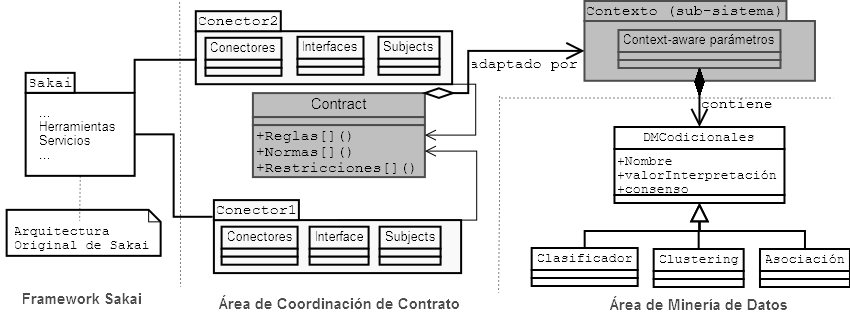
\includegraphics[width=6 in,totalheight=2 in]{Ch4/f3.png}
 % .: 0x0 pixel, 0dpi, nanxnan cm, bb=
\end{center}
\caption{Modelo de integración de los MDCondicionales}
\end{figure}


En las secciones posteriores nos introduciremos en las propuestas y justificaciones
para la incorporación de las técnicas de minería de datos a través
de los \textit{MDcondicional}.

Algoritmos de construcción de los \textit{MDcondicionales} Una de las formas más
simples
de representar conocimiento es mediante árboles de decisión. Dicha estructura de
representación del conocimiento está formada por una serie de nodos, donde: cada
nodo interno es etiquetado con el nombre de uno de los atributos predictores;
las ramas que salen de un nodo interno son etiquetadas con los valores del
atributo de ese nodo; cada nodo terminal, o nodo hoja, es etiquetado con el
valor del atributo objetivo.

Un ejemplo de árbol de decisión se muestra en la figura 4, donde el
atributo objetivo es el atributo nivel de aceptación y los atributos predictores
son lo atributos: interacción, respuestas, evaluación, consultas. Una
característica muy interesante de los árboles de decisión es que, a
partir de ellos, es muy fácil derivar un conjunto de reglas de producción del
tipo Si-entonces (If-Then) completamente equivalente al árbol original. El
algoritmo que nos permite realizar este cambio de modelo de representación
es casi trivial y convierte cada camino que va desde el nodo raíz hasta una
hoja, en una regla de la siguiente forma: los nodos internos y sus correspondientes
ramas de salida son convertidos en las condiciones del antecedente de la regla; los nodos hojas se convierten en el consecuente de la regla. Al convertir el árbol de decisión en una colección de reglas se obtiene una regla por hoja del árbol. Dichas reglas serán, por tanto, mutuamente excluyentes.

El algoritmo de construcción de árboles de decisión más popular es el algoritmo ID3 (Quinlan, J. R., 1987). Este algoritmo está basado en la división sucesiva y construye el árbol de decisión desde la raíz hacia las hojas, incrementando en cada paso la complejidad del árbol.

Inicializar T con el conjunto de todas las instancias Si (todas las instancias en el conjunto T satisfacen el criterio de parada) Entonces Crear un nodo hoja etiquetado con el nombre de la clase y  parar.

Sino Seleccionar un atributo para utilizar como atributo de particionado.
Crear un nodo etiquetado con el nombre del atributo y crear una rama por cada valor del atributo.
Particionar T en subconjuntos tales que contengan las instancias que cumplan los valores del atributo.

Aplicar este algoritmo recursivamente para cada subconjunto.
Fin Si Recorrer el árbol y formar las reglas.


\subsubsection{Modelo de integración}

Para lograr la incorporación de la componente data mining, volvemos a proponer
una nueva integración a muy bajo costo, desde el punto de vista del
rediseño e implementación con el propósito de facilitar la misma y el impacto
en la modificación de los módulos estándares de la aplicación e-learning. En
particular, Sakai, a diferencia de Moodle, provee una arquitectura en la que es
posible trabajar bajo el paradigma orientado a objetos (POO), con toda la
potencia y versatilidad de la tecnología Java, motivo por el cual se logra una
mejor adaptación del modelo de la componente conceptual data mining
mediante un correcto diseño orientado a objeto (DOO) (Grady, B., 1982).
En la figura 5, representamos el contrato con un diagrama de clase. Las
reglas, normas y restricciones (RNR) están representadas con tres métodos
independientes en el diagrama de la clase contrato.
Teniendo en cuenta la analogía planteada entre las reglas del contrato y la
estructura de los árboles que determina el algoritmo TDIDT, es posible plantear
un nuevo mecanismo total o parcial de construcción de reglas dentro de los
contratos. Esta nueva perspectiva puede ser conceptualizada de las siguientes
formas: 1) el uso de técnicas de data mining permite una construcción automática
de reglas. Bajo los contratos (representado en la figura 5 como una
relación de agregación en UML) se realiza dicha construcción en tiempo de
ejecución. En este caso se aporta automatización, adaptabilidad y dinamismo;
2) proporciona una manera indirecta de recolección de información de contexto,
debido a la naturaleza de este tipo de técnicas (minería de datos) donde
la fuente de información procesada reviste a datos empíricos y valores que
denotan tipos de relaciones. Con esta información de contexto, los contratos
adquieren mayores niveles expresivos en cuanto a su sensibilidad al contexto,
similar a los sistemas context-aware.


\begin{center}
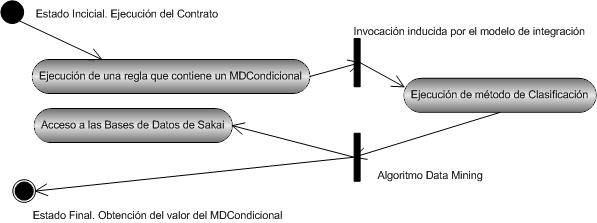
\includegraphics[width=6 in,totalheight=2 in]{Ch4/f4.jpg}
 % .: 0x0 pixel, 0dpi, nanxnan cm, bb=
\caption {Ejecución ****}
\label{fig:ejecucion}
\end{center}



Cuando, dentro en una NRR se utiliza un método para implementar
algunas de las técnicas de data mining (en este caso, la construcción de un
árbol de decisión por medio de un algoritmo TDIDT), queda conformada una
regla donde el valor de su condicional (el cual fue denominado MDcondicional)
responde –conceptualmente– a una estructura, en este caso: un árbol.
El vínculo entre las reglas del contrato y la efectiva representación del TDIDT
se concreta a través de una relación de agregación entre los parámetros del
contrato (representado por la clase “parámetros context-aware”, que se encuentra
dentro del subsistema que engloba el contexto, similar a la propuesta de
Schmidt, A., 2005) y la clase DMcondicionales (representada como una
generalización de subclases donde se distinguen las posibles técnicas de data
mining).

En la figura \ref{}, las componentes significativas para la integración de los
modelos se encuentran enmarcadas en color gris. La primera pertenece al área
de coordinación de contrato y mantiene la estructura original del modelo pro-

puesto en el proyecto “Obra abierta”. La segunda componente se encuentra
representada por una clase conceptual que simboliza las características y funcionalidades
de minería de datos, articuladas para cumplir los objetivos y
requerimientos propuestos.

\paragraph{Mecanismo de comunicación}

La figura 5 es una reelaboración significativa de integración arquitectónica
entre dos modelos (el framework e-learning y el modelo de minería de datos)
donde se muestran, además, relaciones salientes de dependencias entre objetos
de las distintas áreas. Por ejemplo, cuando un objeto perteneciente a una
herramienta5 de la aplicación atiende un pedido de un usuario, se comunica
con otro objeto (en este caso un objeto contrato, perteneciente al área de
coordinación de contrato) con el propósito de verificar la existencia de una
regla que determine cuáles son las acciones que se deben tomar, teniendo en
cuenta determinadas condiciones. Si alguna de las condiciones está representada
por un MDcondicional, entonces existirá una comunicación entre el
objeto contrato (que contiene la regla) y un objeto del área de minería de
datos. Esta cadena de eventos y relaciones entre áreas permite que un servicio
ordinario del framework Sakai se pueda enriquecer con información de contexto
recopilada con técnicas de minería de datos.

\paragraph{Caso de uso}

Retomamos un requerimiento similar al propuesto en la sección “Métricas
de interacción para ‘Obra abierta’ ”, y agregamos que el análisis de información
almacenada es utilizada como recompilación de información (datos) de
contexto.

En este ejemplo, cambiaremos pequeños aspectos de los requerimientos
originales para poder involucrar las técnicas de minería de datos como parte
de la implementación, refiriendo el caso sobre el entorno Sakai.
Supongamos ahora que volvemos a la hipótesis de contar con un dispositivo
hipermedial conformado con la arquitectura del modelo de integración y
además, la implementación del modelo de la figura 6. Sabemos que la herramienta
se encuentra configurada con un contrato (del tipo de la sección “Los
contratos context-aware”) conformado, a su vez, con una regla similar a la presentada
en la sección “Modelo de integración”.

Entonces, cuando un usuario alumno ingrese al foro y ejecute cualquier
tipo de servicios donde intervenga el contrato anterior, las prestaciones que
recibirá estarán supeditadas a los valores que se obtengan de la ejecución del
clasificador en base a la información obtenida a partir del registro de actividades
de la plataforma Sakai. Cabe aclarar que Sakai contiene un registro de
actividades al cual podemos acceder desde las tablas de las bases de datos.
La implementación y operatoria que implique la clasificación de los
datos desde los \textit{MDcondicionales} es responsabilidad del subsistema que
lo
implementa, respetando de esta manera la propiedad de independencia entre
los modelos de la integración señalada en la sección “Detalles del modelo de
integración”.

Si profundizamos en el tipo de relación que se establece a través de los
\textit{MDcondicionales} y tomamos como referencia el punto de vista del
usuario,
podemos caracterizar el flujo de ejecución de órdenes de la siguiente manera:
en la figura 6, podríamos considerar un estado inicial, en el que el sistema ejecuta
las reglas de un contrato que contiene una de ellas con un
\textit{MDcondicional}. Por medio de un método, se produce la invocación del
método
de clasificación que se encuentra implementado en el subsistema de minería
de datos (referenciado con la entidad “modelo externo” en la sección “El
contrato como conector”).

Las transacciones y estados que se suscitan son luego transparentes para el
modelo de integración y pueden resumirse en la ejecución de un algoritmo de
data mining donde se provoca un consulta a la base de datos Sakai y la ejecución
de métodos de clasificación (similares a los de la sección “Antecedentes
de técnicas de minería de datos”) para obtener el valor de verdad del
\textit{MDcondicional}, llegando, así, al estado final del ciclo de ejecución.


Con este tipo de configuración, la herramienta foro de Sakai adquiere
características context-aware y el agregado de la siguiente propiedad: los contratos
context-aware pueden ser modificados en tiempo de ejecución. Esto
quiere decir, que el mismo alumno, ante una nueva interacción con el foro y
bajo las mismas condiciones, puede obtener resultados diferentes en el caso de
que se hayan modificado las reglas del contrato. Además, la incorporación de
un subsistema para la aplicación de técnicas de minería de datos ofrece mayor
potencial expresivo para la construcción de reglas en los contratos.


Finalmente, sobre esta temática consideramos que el uso de un correcto
modelo para la implementación de técnicas de minería en la clasificación de
valores de contextos permite potenciar las soluciones creadas para los dispositivos
hipermediales dinámicos para educación e investigación. Es importante
entonces, que el grupo de diseñadores, expertos y desarrolladores sean competentes
en la utilización comprensiva de este tipo de técnicas.

\begin{center}
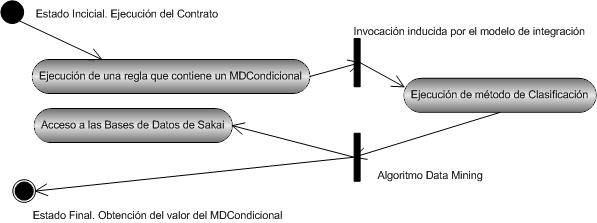
\includegraphics[width=6 in,totalheight=2 in]{Ch4/f4.jpg}
 % .: 0x50380343 pixel, 0dpi, 0.00xinf cm, bb=
\end{center}


\subsetion {Hacia la implementación de los CondicionalesDHD}

Con el objetivo de profundizar la visión sobre el diseño de dispositivos hipermediales
dinámicos, abordamos en este capítulo especificaciones técnicas que
justificaron la implementación y diseño de modelos de integración donde la
componente contrato adoptaba el rol de conector.
Observamos, entonces, que la base conceptual para que el contrato pueda
ser visto y manipulado en su diseño e implementación como una pieza de software,
se centra en el rol protagónico y responsable que debemos adoptar como
expertos diseñadores de dispositivos hipermediales dinámicos en el ciclo de
vida del mismo (diseño, implementación, uso).

Es a partir de esta nueva toma de posición, que la etapa de diseño adquiere
una dimensión activa centrada en la participación con la puesta en obra de
la teoría de coordinación de contratos context-aware.

Tomamos conciencia de que el camino hacia la implementación del
marco teórico propuesto demanda detenimiento para su comprensión, integración
de conocimientos de distintas disciplinas, diálogo interdisciplinar
para poder alcanzar claros criterios en la utilización del contrato y en la explicitación
de las reglas singulares que lo componen, configuradas en función de
los procesos educativos, investigativos o de producción que las susciten.
Teniendo en cuenta su poder expresivo, podremos desarrollar adecuadas
aplicaciones contextualizadas que nos abran la posibilidad de desarrollar nuestra
formación continua y creatividad, construyendo polifónicamente una singular
mesa de arena.


\section{Conclusiones}


ffsdffsdfsdfds


